\documentclass[12pt,oneside]{article}

% Ładujemy Twój szablon
\usepackage{szablon_pokrywka}

% --- KONFIGURACJA DANYCH ---
\author{Mateusz Pokrywka}
\studentID{177143}
\type{Dokumentacja Projektu} % Np. Projekt Inżynierski, Sprawozdanie
\course{Systemy wbudowane}
\title{System kaskady zbiorników do mieszania lakierów samochodowych}

% Opcjonalnie: zmiana ścieżki do loga, jeśli nie jest w figures/
% \setlogopath{logoweii.jpg}

\begin{document}

% 1. Strona tytułowa
\maketitle

% 2. Spis treści
\tableofcontents
\clearpage

\section{Opis projektu}
Projekt polega na implementacji kaskady zbiorników do mieszania lakierów samochodowych. System umożliwia tworzenie dwóch rodzajów lakierów: akrylowego i poliuretanowego, poprzez mieszanie dwóch składników: bazy i utwardzacza. Proporcje składników są zgodne z realnym procesem produkcyjnym - 2:1 dla lakieru akrylowego i 4:1 dla poliuretanowego. Cały proces tworzenia lakieru został zwizualizowany poprzez użycie symulatora.

\section{Realny proces produkcji}
Chcąc zachować spójność z prawdziwym procesem produkcyjnym, kaskada została zaprojektowana tak, aby w jak najwyższym stopniu odzwierciedlać rzeczywiste proporcje. Baza i utwardzacz są napełniane, podgrzewane i utrzymywane w gotowości zgodnie z wymaganiami technologicznymi. Mieszanie odbywa się przez określoną liczbę cykli, a temperatura gotowej mieszaniny jest kontrolowana, aby zapewnić odpowiednią jakość lakieru. System jest również wyposażony w zabezpieczenia, które chronią przed przelaniem, przegrzaniem oraz pracą elementów wykonawczych bez cieczy w zbiornikach.\\
Poniższe zdjęcia z kart katalogowych producentów lakierów ilustrują proporcje miaszania:
\begin{figure}[H]
    \centering
    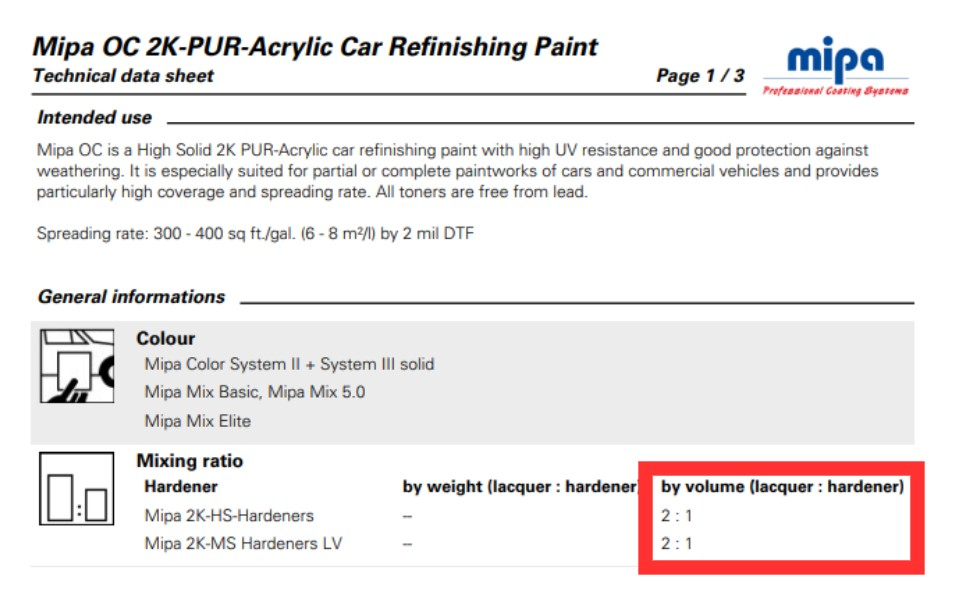
\includegraphics[width=14cm]{figures/ss_zbiorniki/teoria_akryl.jpg}
    \caption{Karta katalogowa lakieru akrylowego Mipa OC 2K-PUR-Acrylic Car Refinishing Paint}
    \label{Fig:tech_akryl}
\end{figure}

\begin{figure}[H]
    \centering
    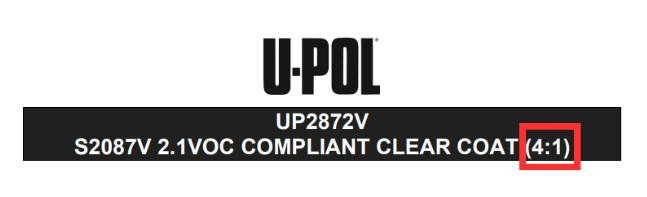
\includegraphics[width=14cm]{figures/ss_zbiorniki/teoria_poliu.jpg}
    \caption{Karta katalogowa lakieru poliuretanowego UP2872VS2087V 2.1VOC COMPLIANT CLEAR COAT (4:1)}
    \label{Fig:tech_poliu}
\end{figure}

\section{Założenia szczegółowe}
\begin{itemize}
    \item Zbiornik nr 1 - baza
    \begin{enumerate}
        \item Napełnianie do poziomu x2
        \item Grzanie do temperatury 30°C oraz dogrzewanie przez dokładnie 160 cykli
        \item Oczekiwanie w gotowości i podtrzymywanie temperatury do czasu obniżenia poziomu bazy poniżej x1
    \end{enumerate}
    \item Zbiornik nr 2 - utwardzacz
        \begin{enumerate}
        \item Napełnianie do poziomu x3
        \item Dalsze napełnianie do poziomu x4 wraz z grzaniem 
        \item Grzanie do osiągnięcia temperatury 30°C, a następnie dogrzewanie przez dokładnie 160 cykli
        \item Oczekiwanie w gotowości i podtrzymywanie temperatury do czasu obniżenia poziomu utwardzacza poniżej x3
    \end{enumerate}
    \item Zbiornik nr 3 - mieszanina
        \begin{enumerate}
        \item Oczekiwanie na napełnienie i odpowiednią temperaturę górnych zbiorników
        \item Napełnianie bazą 400 cykli oraz utwardzaczem (200 lub 100 cykli w zależności od typu lakieru) 
        \item Mieszanie przez dokładnie 300 cykli
        \item Grzanie mieszaniny do osiągnięcia temperatury docelowej 45°C
        \item Opróżnianie do poziomu x5
    \end{enumerate}
\end{itemize}

\section{Opis UI i funkcjonalności}
Projekt umożliwia dwa podstawowe tryby pracy:
\begin{itemize}
    \item Automatyczny - system działa zgodnie z założonymi regułami maszyny Moore'a (na przemian tworzy lakier akrylowy i poliuretanowy), a użytkownik może obserwować proces.
    \item Manualny - użytkownik ma pełną kontrolę nad wyjściami, może ręcznie sterować napełnianiem, grzaniem i mieszaniem. Ograniczeniem są sprzętowe zabezpieczenia uniemożliwiające przelanie, przegrzanie oraz pracę elementów wykonawczych "na sucho".
\end{itemize}

Sterować kaskadą można za pomocą przełączników i przycisków symulatora, a istotne informacje (aktywny tryb, temperatury, wybrane urządzenia) przedstawione są na wyświetlaczu LCD.

\begin{figure}[H]
    \centering
    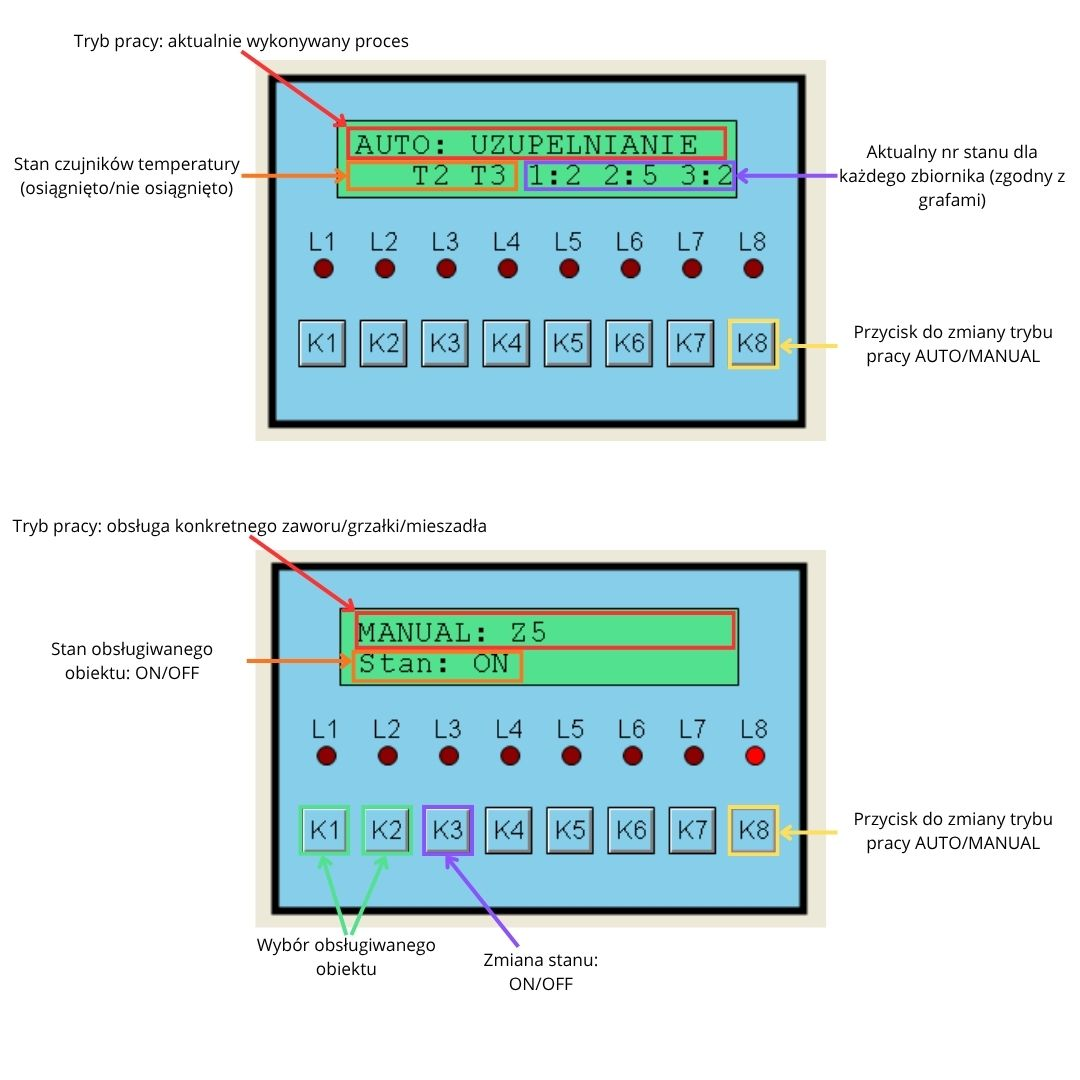
\includegraphics[width=14cm]{figures/ss_zbiorniki/UI.jpg}
    \caption{Opis interfejsu użytkownika}
    \label{Fig:UI}
\end{figure}

\section{Teoretyczne podstawy działania}
\subsection{Zasady}
\begin{itemize}
    \item Zbiornik nr 1 - baza
    \begin{enumerate}
        \item $h < x1$ Napełniaj Z1 do poziomu x2
        \item $x1 < h \ge x2$ Grzej G1 do temperatury T1, a następnie przez dokładnie 160 cykli\\
        Oczekuj na opróżnienie zbiornika do poziomu x1, podtrzymując temperaturę T1
    \end{enumerate}
    \item Zbiornik nr 2 - utwardzacz
    \begin{enumerate}
        \item $h < x3$ Napełniaj Z2 do poziomu x3
        \item $x3 <h \ge x4$ Dalej napełniaj Z2 do poziomu x4, jednocześnie grzejąc G2\\
        Grzej G2 do temperatury T2, a następnie przez dokładnie 160 cykli\\
        Oczekuj na opróżnienie zbiornika do poziomu x3, podtrzymując temperaturę T2
    \end{enumerate}
    \item Zbiornik nr 3 - mieszanina
        \begin{itemize}
            \item Lakier akrylowy:
                \begin{enumerate}
                \item $h < x5$ Napełniaj z Z2/Z4 do poziomu x7 w cyklu 400:200
                \item $h \ge x7$ Mieszaj przez dokładnie 300 cykli\\
                Następnie grzej G3+G4 do osiągnięcia temperatury 45°C\\
                W każdej chwili, jeżeli zabraknie bazy lub utwardzacza, zatrzymaj napełnianie i pulsuj G3 co 300 cykli do momentu uzupełnienia braków\\
                \end{enumerate}
            \item Lakier poliuretanowy:
                \begin{enumerate}
                \item $h < x5$ Napełniaj z Z2/Z4 do poziomu x7 w cyklu 400:100
                \item $h \ge x7$ Mieszaj przez dokładnie 300 cykli\\
                Następnie grzej G3+G4 do osiągnięcia temperatury 45°C\\
                W każdej chwili, jeżeli zabraknie bazy lub utwardzacza, zatrzymaj napełnianie i pulsuj G3 co 300 cykli do momentu uzupełnienia braków\\ 
                \end{enumerate}
        \end{itemize}
         \item Tryb manualny
         \begin{itemize}
            \item W każdym momencie poprzez K8, użytkownik może przejść do trybu ręczego
            \item W momencie przejścia wszystkie do trybu manualnego, wszystkie wyjścia zbiorników zostają wyłączone, a poprzez K1, K1 i K3 użytkownik może ręcznie sterować napełnianiem, grzaniem i mieszaniem
            \item K1, K2 - wybór konkretnego wyjścia
            \item K3 - włączanie/wyłączanie wybranego wyjścia
            \item Cały czas obowiązują sprzętowe zabezpieczenia przed przelaniem, przegrzaniem oraz pracą grzałki bez cieczy w zbiorniku
            \item Po powrocie do trybu automatycznego system opróżnia zbiorniki i rozpoczyna tworzenie ostatniego lakieru od początku
         \end{itemize}
\end{itemize}
\subsection{Przebiegi czasowe}
Przebieg czasowy zbiornika nr 1 - baza:
\begin{figure}[H]
    \centering
    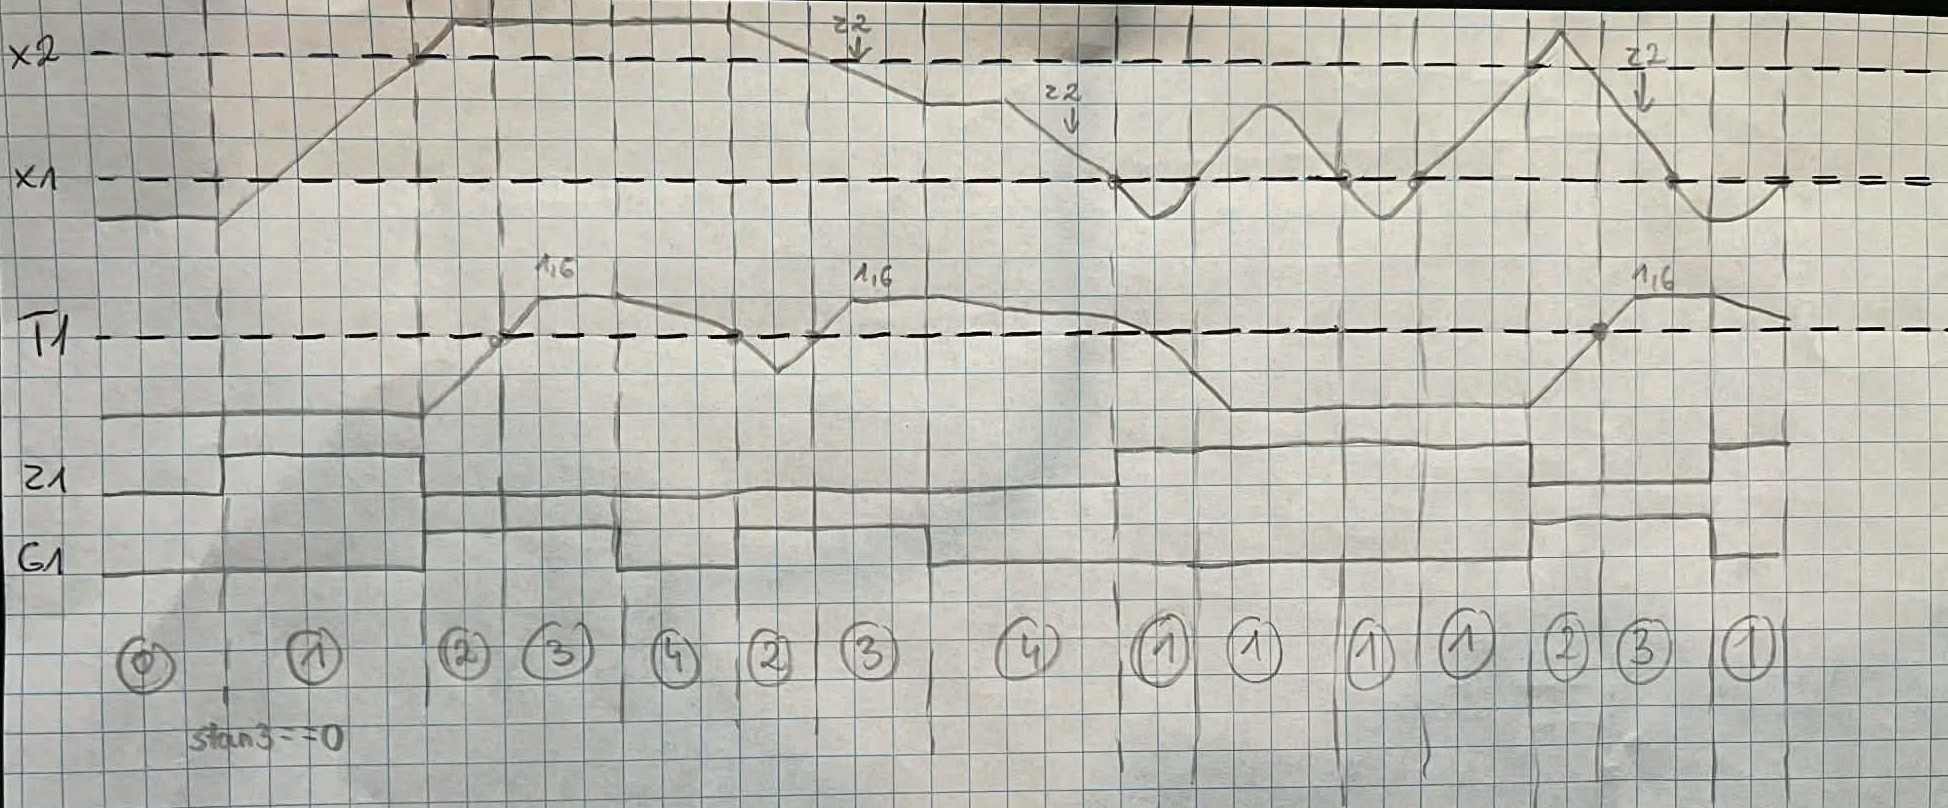
\includegraphics[width=14cm]{figures/skany/p1.jpeg}
    \caption{Przebieg czasowy zbiornika nr 1 - baza}
    \label{Fig:przebieg_z1}
\end{figure}

Przebieg czasowy zbiornika nr 2 - utwardzacz:
\begin{figure}[H]
    \centering
    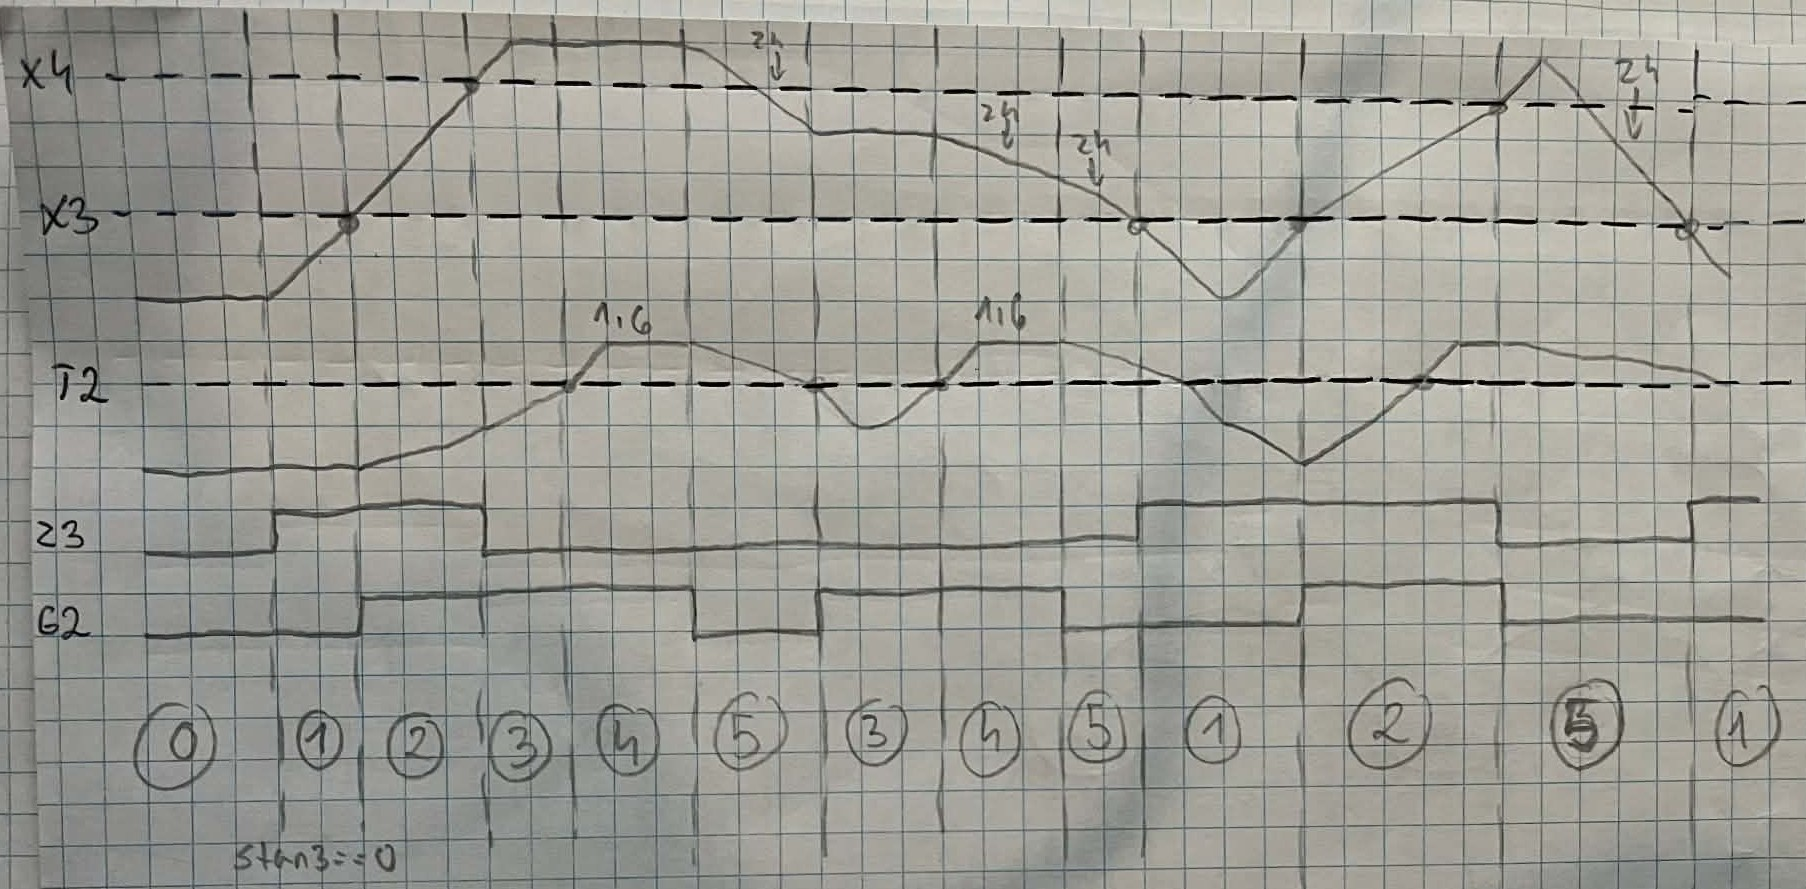
\includegraphics[width=14cm]{figures/skany/p2.jpeg}
    \caption{Przebieg czasowy zbiornika nr 2 - utwardzacz}
    \label{Fig:przebieg_z2}
\end{figure}

Przebieg czasowy zbiornika nr 3 - mieszanina:
\begin{figure}[H]
    \centering
    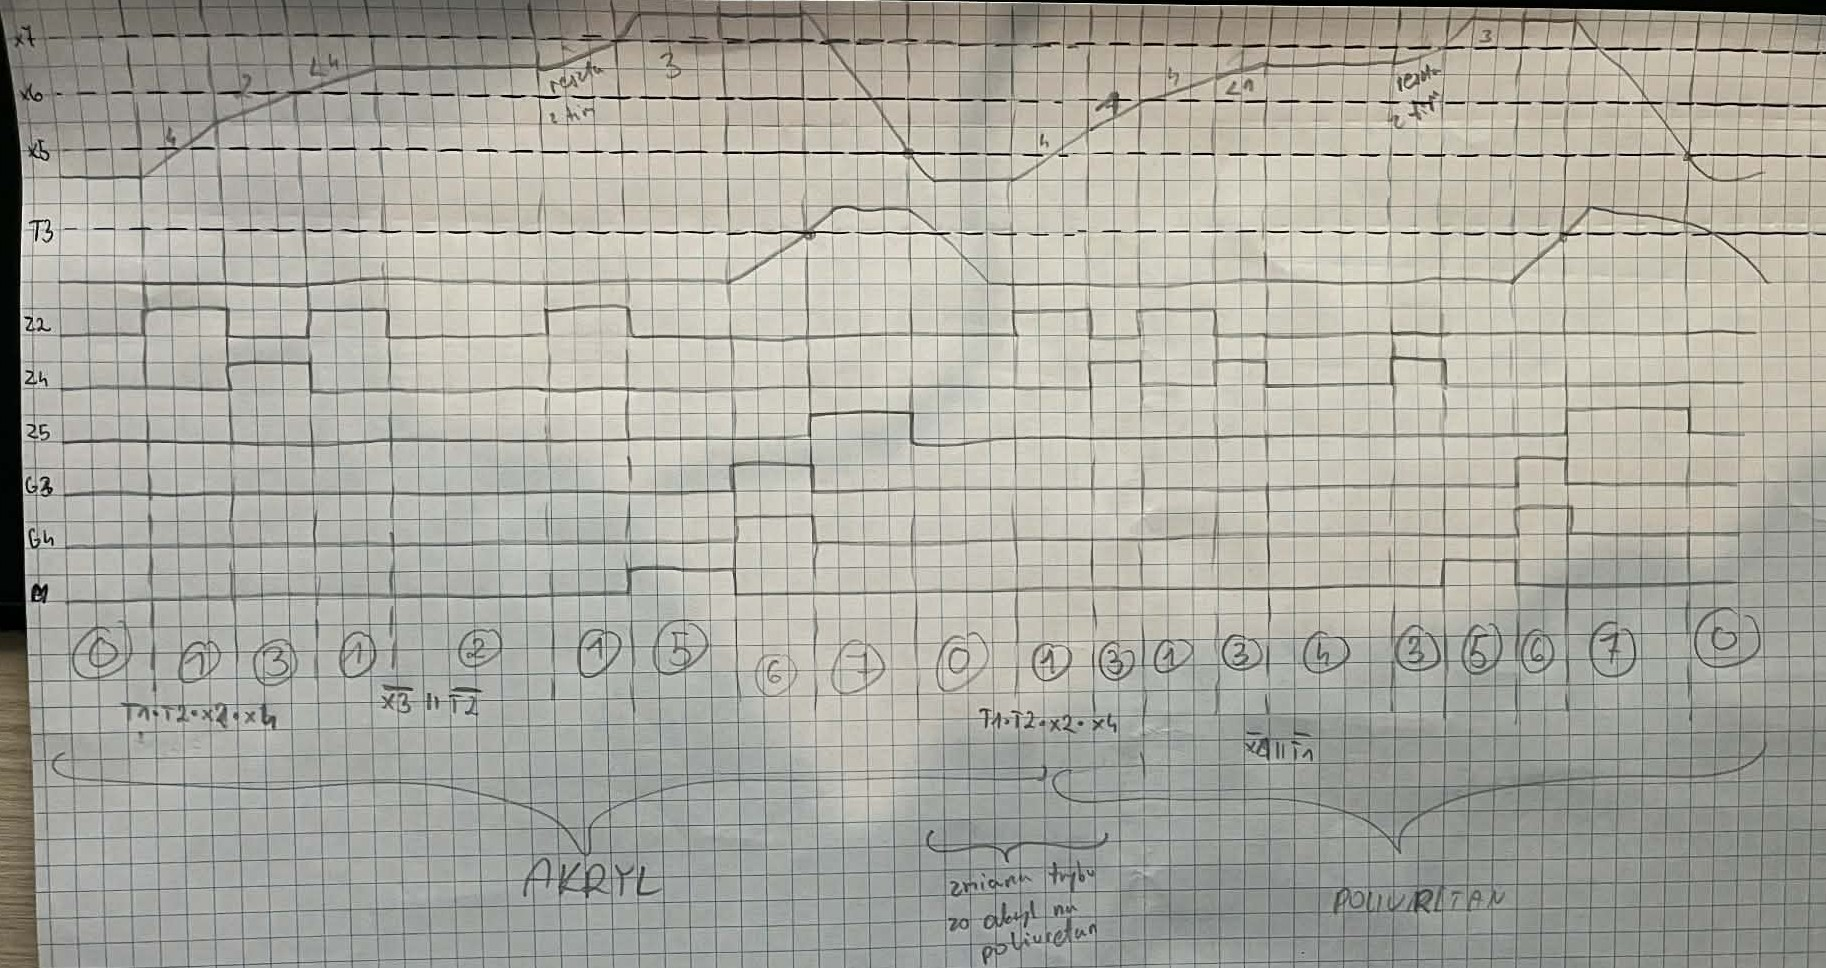
\includegraphics[width=14cm]{figures/skany/p3.jpeg}
    \caption{Przebieg czasowy zbiornika nr 3 - mieszanina}
    \label{Fig:przebieg_z3}
\end{figure}

\subsection{Opisy stanów}
\begin{itemize}
    \item Zbiornik nr 1 - baza
    \begin{itemize}
        \item Stan 0: Oczekiwanie na start oraz gotowość dolnego zbiornika (Z1=0, G1=0)
        \item Stan 1: Napełnianie do poziomu x2 (Z1=1, G1=0)
        \item Stan 2: Grzanie do temperatury T1 (Z1=0, G1=1)
        \item Stan 3: Dogrzewanie przez dokładnie 160 cykli (Z1=0, G1=1)
        \item Stan 4: Oczekiwanie na opróżnienie (Z1=0, G1=0)
    \end{itemize}
    \item Zbiornik nr 2 - utwardzacz
    \begin{itemize}
        \item Stan 0: Oczekiwanie na start oraz gotowość dolnego zbiornika (Z3=0, G2=0)
        \item Stan 1: Napełnianie do poziomu x3 (Z3=1, G2=0)
        \item Stan 2: Napełnianie z grzaniem do poziomu x4 (Z3=1, G2=1)
        \item Stan 3: Grzanie do temperatury T2 (Z3=0, G2=1)
        \item Stan 4: Dogrzewanie przez dokładnie 160 cykli (Z3=0, G2=1)
        \item Stan 5: Oczekiwanie na opróżnienie (Z3=0, G2=0)
    \end{itemize}
    \item Zbiornik nr 3 - mieszanina
    \begin{itemize}
        \item Stan 0: Oczekiwanie na napełnienie górnych zbiorników (Z2=0, Z4=0, Z5=0, M=0, G3=0, G4=0)
        \item Stan 1: Napełnianie bazą przez maksymalnie 400 cykli (Z2=1, Z4=0, Z5=0, M=0, G3=0, G4=0)
        \item Stan 2: Pauza Z2 - brak bazy lub niedogrzanie (Z2=0, Z4=0, Z5=0, M=0, G3 pulsuje co 300 cykli, G4=0)
        \item Stan 3: Napełnianie utwardzaczem maksymalnie 200 lub 100 cykli w zależności od rodzaju lakieru (Z2=0, Z4=1, Z5=0, M=0, G3=0, G4=0)
        \item Stan 4: Pauza Z4 - brak utwardzacza lub niedogrzanie (Z2=0, Z4=0, Z5=0, M=0, G3 pulsuje co 300 cykli, G4=0)
        \item Stan 5: Mieszanie dokładnie 300 cykli (Z2=0, Z4=0, Z5=0, M=1, G3=0, G4=0)
        \item Stan 6: Grzanie G3+G4 do 45°C (Z2=0, Z4=0, Z5=0, M=0, G3=1, G4=1)
        \item Stan 7: Opróżnianie do poziomu x5 (Z2=0, Z4=0, Z5=1, M=0, G3=0, G4=0)
        \item Stan 8: Zerowanie układu po trybie MANUAL (Z2=1, Z4=1, Z5=1, M=0, G3=0, G4=0)
        \item Stan 9: Dalsze zerowanie (Z2=0, Z4=0, Z5=1, M=0, G3=0, G4=0)
    \end{itemize}
\end{itemize}
\subsection{Grafy stanów}
Graf stanów zbiornika nr 1 - baza:
\begin{figure}[H]
    \centering
    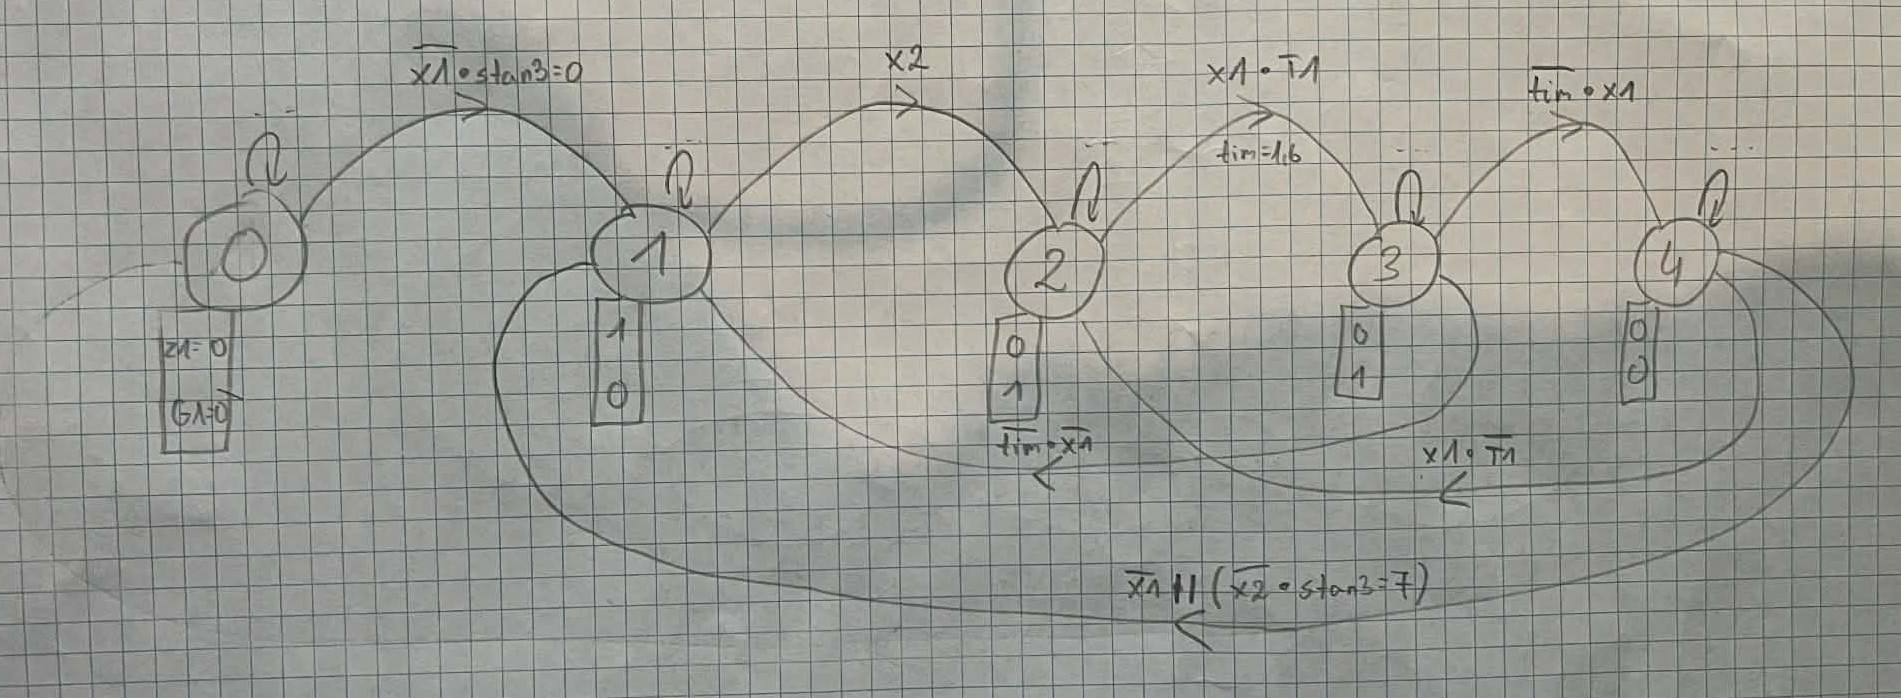
\includegraphics[width=14cm]{figures/skany/g1.jpeg}
    \caption{Graf stanów zbiornika nr 1 - baza}
    \label{Fig:graf_z1}
\end{figure}

    Graf stanów zbiornika nr 2 - utwardzacz:
\begin{figure}[H]
    \centering
    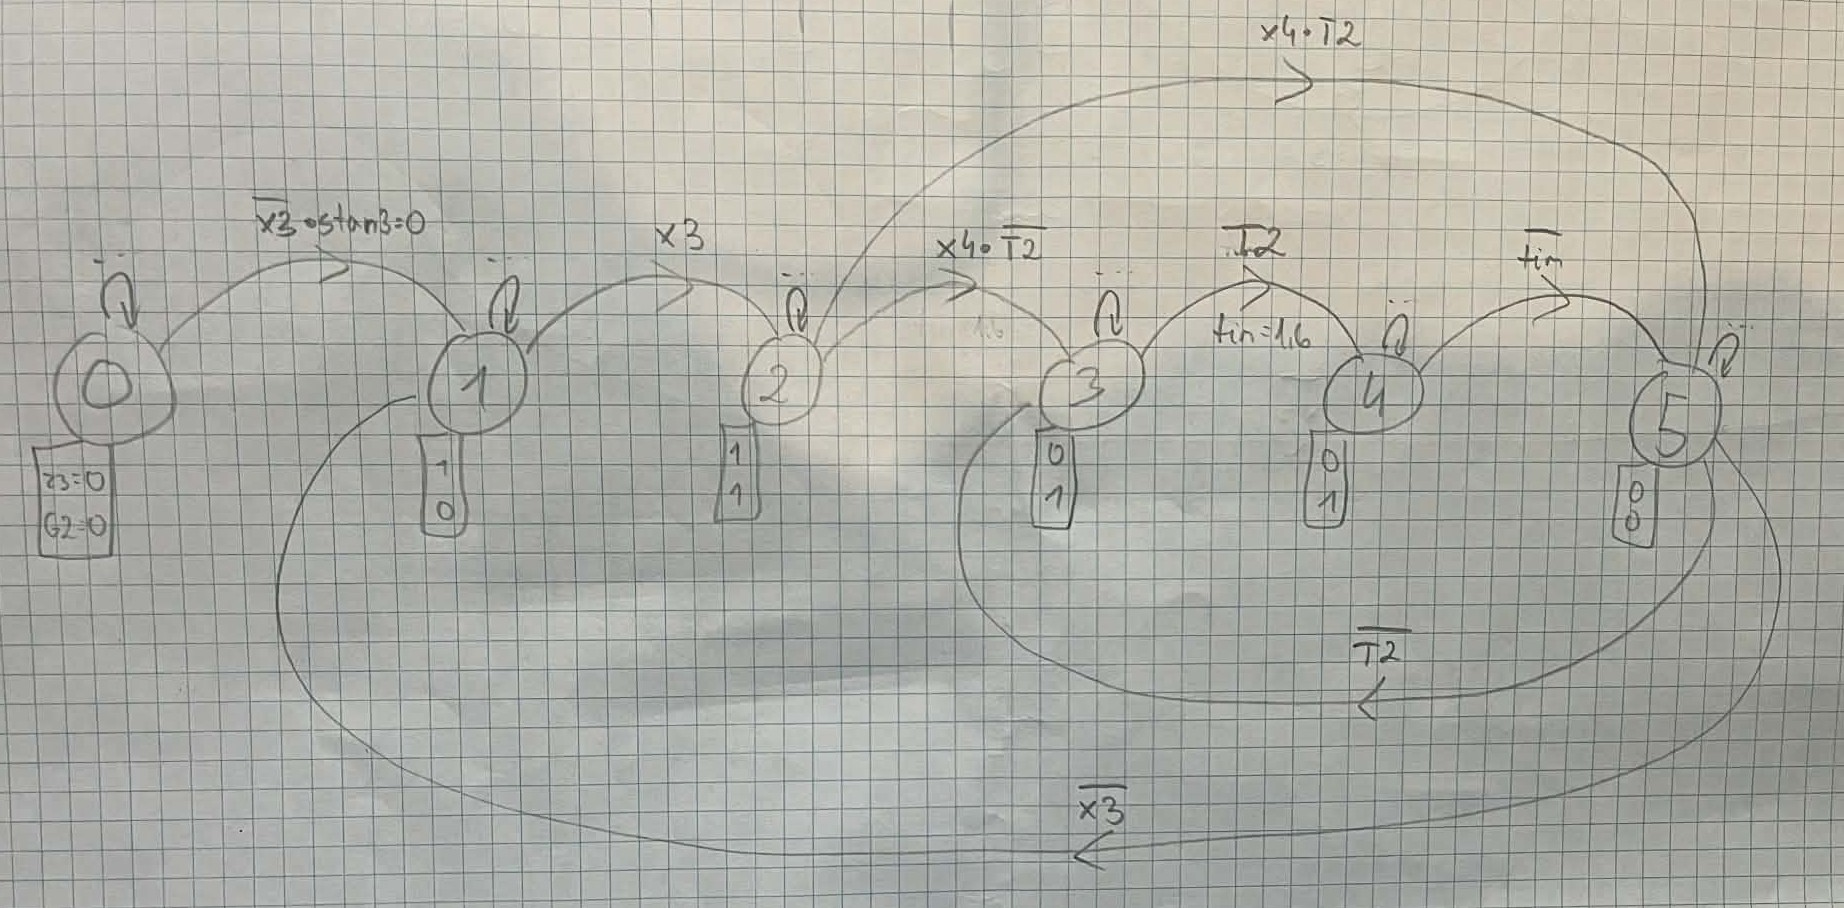
\includegraphics[width=14cm]{figures/skany/g2.jpeg}
    \caption{Graf stanów zbiornika nr 2 - utwardzacz}
    \label{Fig:graf_z2}
\end{figure}

    Graf stanów zbiornika nr 3 - mieszanina:
\begin{figure}[H]
    \centering
    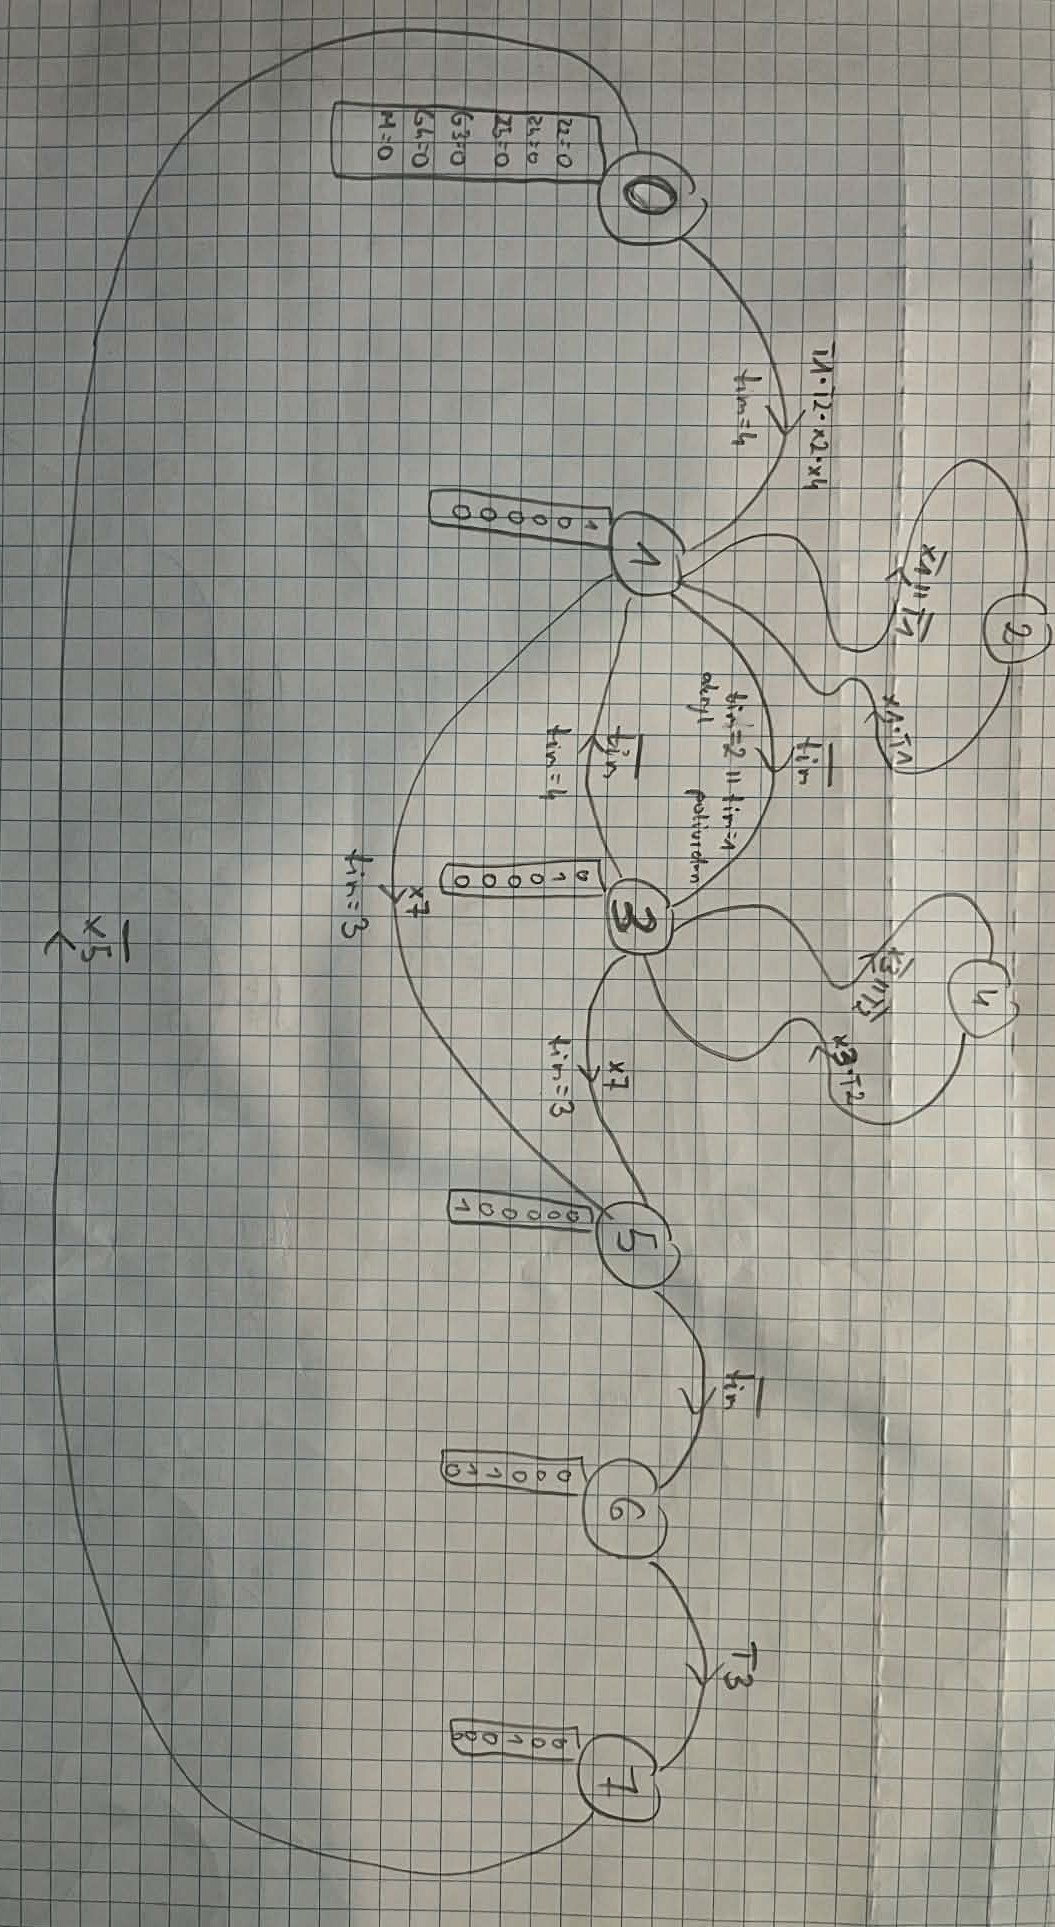
\includegraphics[width=14cm]{figures/skany/g3.jpeg}
    \caption{Graf stanów zbiornika nr 3 - mieszanina}
    \label{Fig:graf_z3}
\end{figure}

\section{Implementacja kodu}
\begin{lstlisting}[language=C, caption={Definicja zmiennych}, label={Kod:Definicja}]
int licz;                   // Licznik cykli
int tim1, tim2, tim3;       // Timery

char stan1, stan2, stan3;   // Aktualny stan
int tryb, nastepny_tryb;    // Aktualny rodzaj lakieru (1 - akrylowy, 2 - poliuretanowy) oraz zmienna pomocnicza do jego przechowywania podczas przejścia do trybu manualnego

float temp1, temp2, temp3;  // Aktualna temperatura w zbiornikach
float T1_set, T2_set, T3_set; // Docelowe wartości temperatur (aktywacja czujników temperatury)

// Makra ułatwiające sprawdzanie, czy docelowa temperatura w danym zbiorniku została osiągnięta
#define T1 (temp1 >= T1_set) // Zwraca prawde, gdy temp. w zbiorniku 1 osiagnie zadaną
#define T2 (temp2 >= T2_set) // Zwraca prawde, gdy temp. w zbiorniku 2 osiagnie zadaną
#define T3 (temp3 >= T3_set) // Zwraca prawde, gdy temp. w zbiorniku 3 osiagnie zadaną

// Zmienne do trybu manualnego i pauz
int timer_pauzy;            // Licznik pomocniczy służący do pulsowania grzałki G3 podczas pauzy 
int man_wybor;              // Zmienna przechowująca indeks aktualnie wybranego urządzenia w menu trybu manualnego (od 0 do 9)
char man_out[10];           // Tablica przechowująca żądane stany wyjść (ON/OFF) ustawione przez użytkownika w trybie manualnym
char KL, prev_KL;           // Zmienne przechowujące aktualny i poprzedni stan przełącznika K8 (służą do wykrywania momentu zmiany trybu AUTO/MANUAL)
char pauza_tim3;            // Flaga logiczna zatrzymująca odliczanie timera tim3, gdy w dolnym zbiorniku brakuje surowca z góry
\end{lstlisting}

\begin{lstlisting}[language=C, caption={Inicjalizacja zmiennych}, label={Kod:Inicjalizacja}]
void prolog(void) {
    int i; // Zmienna pomocnicza używana jako licznik w pętli for
    
    //Zerowanie wszystkich wyjść cyfrowych (Z1-Z5, G1-G4, M) na początku programu
    L1=L2=L3=L4=L5=L6=L7=L8=0; 
    
    // Synchronizacja stanów "poprzednich" (pK) z "aktualnymi" (aK) dla przycisków/przełączników.
    pK1=aK1; pK2=aK2; pK3=aK3; pK4=aK4;
    pK5=aK5; pK6=aK6; pK7=aK7; pK8=aK8;
    
    //Inicjalizacja zmienncyh
    licz = 0;                         
    tim1 = 0; tim2 = 0; tim3 = 0;     
    
    // Ustawienie stanów początkowych dla grafów stanów zbiorników
    stan1 = 0;                        
    stan2 = 0;                        
    stan3 = 8;                        
    
    tryb = 0;                         // Wyzerowanie aktualnie produkowanego trybu lakieru
    nastepny_tryb = 1;                // Zdefiniowanie, że pierwszym wyprodukowanym lakierem po starcie będzie Akryl (tryb 1)
    
    T1_set = 30.0;                    // Ustawienie docelowej temperatury grzania dla bazy 
    T2_set = 30.0;                    // Ustawienie docelowej temperatury grzania dla utwardzacza 
    T3_set = 45.0;                    // Ustawienie docelowej temperatury grzania dla gotowej mieszaniny 
    
    timer_pauzy = 0;                  // Wyzerowanie licznika odpowiadającego za pulsowanie grzałki podczas pauz
    man_wybor = 0;                    // Ustawienie "kursora" w menu manualnym na pierwszej pozycji (Z1)
    KL = 0; prev_KL = 0;              // Wyzerowanie flag przełącznika trybu AUTO/MANUAL (praca zaczyna się w trybie automatycznym)
    pauza_tim3 = 0;                   // Wyzerowanie flagi wstrzymującej odliczanie czasu w dolnym zbiorniku
    
    // Wyzerowanie bufora wyjść dla trybu manualnego
    for(i = 0; i < 10; i++) man_out[i] = 0; 
}
\end{lstlisting}

\begin{lstlisting}[language=C, caption={Logika symulacji}, label={Kod:Sym}]
    // Tablica nazw wyjść, używana do wyświetlania na LCD informacji w trybie manualnym
    char* nazwy[] = {"Z1", "Z2", "Z3", "Z4", "Z5", "G1", "G2", "G3", "G4", "M"};
    
    //Tablica stanów, używana do przechowywania aktualnych stanów wyjść (ON/OFF) w trybie manualnym
    int stany[10];
    
    //Tablica znaków używana przez funkcję sprintf() do posklejania zmiennych i tekstu w jeden string, zanim wyśle go na ekran.
    char bufor_pomocniczy[30];
    
    // Zmienna pomocnicza do iteracji w pętli for
    int i;


    // Odczyt temperatur z symulatora
    temp1 = AI[0] / 10.0; 
    temp2 = AI[1] / 10.0; 
    temp3 = AI[2] / 10.0; 

    // Odczyt K8 z panelu
    KL = aK8; 
    
    // Sygnalizacja trybu manualnego poprzez diodę L8
    L8 = aK8;

    // Wykrywanie zmiany stanu przełącznika K8 (AUTO/MANUAL)
    if (KL && !prev_KL) {
        // Przejście do trybu manualnego - wyzerowanie wszystkich wyjść i stanów automatów
        for(i = 0; i < 10; i++) man_out[i] = 0;
        
        // Zatrzymanie wszystkich procesów - wyłączenie grzania, mieszania i napełniania
        stan1 = 0; stan2 = 0; stan3 = 8; 
        tryb = 0; // Skasowanie zapamiętanego wyboru lakieru
    }
}
\end{lstlisting}

\begin{lstlisting}[language=C, caption={Tryb manualny}, label={Kod:Man}]
  if (KL) {
        // Logika wyboru urządzenia w menu manualnym
        if (aK1 != pK1) { man_wybor--; if (man_wybor < 0) man_wybor = 9; }
        if (aK2 != pK2) { man_wybor++; if (man_wybor > 9) man_wybor = 0; }
        
        // Logika włączania/wyłączania wybranego urządzenia
        if (aK3 != pK3) { man_out[man_wybor] = !man_out[man_wybor]; }

        //Zabezpieczenia sprzętowe
        Z1 = (man_out[0] && !x2) ? 1 : 0; 
        Z2 = (man_out[1] && !x7) ? 1 : 0; 
        Z3 = (man_out[2] && !x4) ? 1 : 0; 
        Z4 = (man_out[3] && !x7) ? 1 : 0; 
        Z5 = man_out[4];
        M  = man_out[9];
        G1 = (man_out[5] && x1 && temp1 < T1_set + 15.0) ? 1 : 0;
        G2 = (man_out[6] && x3 && temp2 < T2_set + 15.0) ? 1 : 0;
        G3 = (man_out[7] && x5 && temp3 < T3_set + 15.0) ? 1 : 0;
        G4 = (man_out[8] && x5 && temp3 < T3_set + 15.0) ? 1 : 0;

        // Aktualizacja tablicy stanów dla wyświetlacza LCD
        stany[0]=Z1; stany[1]=Z2; stany[2]=Z3; stany[3]=Z4; stany[4]=Z5;
        stany[5]=G1; stany[6]=G2; stany[7]=G3; stany[8]=G4; stany[9]=M;

        // Formatowanie pierwszej linii ekranu LCD, wstawiając nazwę aktualnie wybranego urządzenia w menu manualnym.
        sprintf(bufor_pomocniczy, "MANUAL: %s", nazwy[man_wybor]);
        sprintf(buf, "%-20s", bufor_pomocniczy); 
        LCD_xy(1,1); LCD_puts(buf);

        // Formatowanie drugiej linii ekranu LCD, wstawiając faktyczny stan (ON/OFF) urządzenia.
        sprintf(bufor_pomocniczy, "Stan: %s", stany[man_wybor] ? "ON" : "OFF"); 
        sprintf(buf, "%-20s", bufor_pomocniczy);
        LCD_xy(1,2); LCD_puts(buf);
        
        Sygnalizacja wciśnięcia przycisków K1-K3 poprzez diody L1-L3
        L1=aK1; L2=aK2; L3=aK3; 
        L4=0; L5=0; L6=0; L7=0; // Zgaszenie nieużywanych diod

    } else { /* Logika trybu automatycznego (następne listingi)*/ }
}
\end{lstlisting}

\begin{lstlisting}[language=C, caption={Tryb automatyczny}, label={Kod:Auto}]
    /*Blok kodu Manualnego (poprzedni listing)*/
    } else {
        //Zgasznie wszystkich diod
        L1=0; L2=0; L3=0; L4=0; L5=0; L6=0; L7=0;
        
        // Wyzerowanie flagi pauzy timera tim3, która jest aktywowana, gdy w dolnym zbiorniku brakuje surowca z góry.
        pauza_tim3 = 0;

        // Logika aktywacji pauzy timera tim3, gdy w dolnym zbiorniku brakuje surowca z góry.
        if (stan3 == 2 || stan3 == 4) { 
            timer_pauzy++; 
            if (timer_pauzy > 600) timer_pauzy = 0; 
        } else { 
            timer_pauzy = 0; 
        }

        /* [...] Tutaj znajdują się 3 bloki switch dla grafów (następne listingi) */

       // Wyświetlanie informacji na LCD
        if (stan3 == 8 || stan3 == 9) {
            sprintf(bufor_pomocniczy, "AUTO: ZEROWANIE");  // Trwa opróżnianie po powrocie z pracy maualnej
        } else if (stan3 == 0 || stan3 == 2 || stan3 == 4) { 
            sprintf(bufor_pomocniczy, "AUTO: UZUPELNIANIE"); // Kaskada czeka, aż górne zbiorniki przygotują bazę/utwardzacz
        } else if (tryb == 1) {
            sprintf(bufor_pomocniczy, "AUTO: AKRYL");        // Trwa normalna produkcja lakieru akrylowego
        } else if (tryb == 2) {
            sprintf(bufor_pomocniczy, "AUTO: POLIURETAN");   // Trwa normalna produkcja lakieru poliuretanowego
        } else {
            sprintf(bufor_pomocniczy, "AUTO: CZEKA");        // Stan przejściowy
        }
        
        // Formatowanie pierwszej linii ekranu LCD, wstawiając aktualny tryb pracy systemu.
        sprintf(buf, "%-20s", bufor_pomocniczy);
        LCD_xy(1,1); LCD_puts(buf); // Wyświetlenie na pierwszej linii (x=1, y=1)
        
       // Formatowanie drugiej linii ekranu LCD, wstawiając aktualne informacje czy temperatura została osiągnięta (T1, T2, T3) oraz aktualne stany zbiorników (stan1, stan2, stan3).
        sprintf(bufor_pomocniczy, "%s %s %s 1:%d 2:%d 3:%d", 
                T1 ? "T1" : "  ",   // Jeśli temp1 >= T1_set, pokaż "T1", inaczej dwie spacje
                T2 ? "T2" : "  ", 
                T3 ? "T3" : "  ",
                (int)stan1, (int)stan2, (int)stan3);
                
        sprintf(buf, "%-20s", bufor_pomocniczy);
        LCD_xy(1,2); LCD_puts(buf); // Wyświetlenie na drugiej linii (x=1, y=2)
    } 

    // Aktualizacja stanu poprzedniego przełącznika K8, aby wykrywać zmiany w następnym cyklu
    prev_KL = KL;

    // Odliczanie timerów
    if(tim1) --tim1; 
    if(tim2) --tim2; 
    if(tim3 && !pauza_tim3) --tim3;

    // Synchronizacja stanów "poprzednich" (pK) z "aktualnymi" (aK)
    pK1 = aK1; pK2 = aK2; pK3 = aK3; pK4 = aK4;
    pK5 = aK5; pK6 = aK6; pK7 = aK7; pK8 = aK8;
}
\end{lstlisting}

\begin{lstlisting}[language=C, caption={Logika zbiornika nr 1 - baza}, label={Kod:zb1}]
        switch(stan1) {
            case 0: 
                Z1=0; G1=0; 
                if(!x1 && stan3 == 0) stan1 = 1; 
                break;
            case 1: 
                Z1=1; G1=0; 
                if(x2) stan1 = 2; 
                break;
            case 2: 
                Z1=0; G1=1; 
                if(!x1) stan1 = 1; 
                else if(x1 && T1) { tim1 = 160; stan1 = 3; } 
                break;
            case 3: 
                Z1=0; G1=1; 
                if(!tim1 && x1) stan1 = 4; 
                else if(!tim1 && !x1) stan1 = 1; 
                break;
            case 4: 
                Z1=0; G1=0; 
                if(!x1 || (stan3 == 7 && !x2)) stan1 = 1; 
                else if(x1 && !T1) stan1 = 2; 
                break;
        }
\end{lstlisting}

\begin{lstlisting}[language=C, caption={Logika zbiornika nr 2 - utwardzacz}, label={Kod:zb2}]
        switch (stan2) {
            case 0: 
                Z3=0; G2=0; 
                if(!x3 && stan3 == 0) stan2 = 1; 
                break;
            case 1: 
                Z3=1; G2=0; 
                if (x3) stan2=2; 
                break;
            case 2: 
                Z3=1; G2=1; 
                if (!x3) stan2=1; 
                else if (x3 && x4 && !T2) stan2=3; 
                else if (x3 && x4 && T2) stan2=5; 
                break;
            case 3: 
                Z3=0; G2=1; 
                if (!x3) stan2=1; 
                else if (x3 && T2) { tim2=160; stan2=4; } 
                break;
            case 4: 
                Z3=0; G2=1; 
                if (!tim2 && x3) stan2=5; 
                else if (!tim2 && !x3) stan2=1; 
                break;
            case 5: 
                Z3=0; G2=0; 
                if (!x3 || (stan3 == 7 && !x4)) stan2 = 1; 
                else if (x3 && !T2) stan2=3; 
                break;
        }
\end{lstlisting}

\begin{lstlisting}[language=C, caption={Logika zbiornika nr 3 - mieszanina}, label={Kod:zb3}]
        switch (stan3) {
            case 0: 
                Z2=0; Z4=0; Z5=0; M=0; G3=0; G4=0; 
                if (T1 && T2 && x2 && x4) { 
                    tryb = nastepny_tryb; // Ustawianie rodzaju lakieru na przemian
                    tim3 = 400;           
                    nastepny_tryb = (tryb == 1) ? 2 : 1; // Przełączanie na drugi lakier po zakończeniu obecnego
                    stan3 = 1;            
                } 
                break;
                
            case 1: 
                Z2=1; Z4=0; Z5=0; M=0; G3=0; G4=0; 
                if (x7) { tim3 = 300; stan3 = 5; } 
                else if (!x7 && (!x1 || !T1)) stan3 = 2; 
                else if (!x7 && x1 && T1 && !tim3) { 
                    tim3 = (tryb == 1) ? 200 : 100; // Akryl - 200 cykli, Poliuretan - 100 cykli
                    stan3 = 3;
                } 
                break;
                
            case 2: 
                Z2=0; Z4=0; Z5=0; M=0; G3=(timer_pauzy <= 300) ? 1 : 0; G4=0; 
                pauza_tim3 = 1; 
                if (x1 && T1) stan3 = 1; 
                break;
                
            case 3:
                Z2=0; Z4=1; Z5=0; M=0; G3=0; G4=0; 
                if (x7) { tim3 = 300; stan3 = 5; } 
                else if (!x7 && (!x3 || !T2)) stan3 = 4; 
                else if (!x7 && x3 && T2 && !tim3) { 
                    tim3 = 400; 
                    stan3 = 1; 
                } 
                break;
                
            case 4: 
                Z2=0; Z4=0; Z5=0; M=0; G3=(timer_pauzy <= 300) ? 1 : 0; G4=0; 
                pauza_tim3 = 1;    
                if (x3 && T2) stan3 = 3; 
                break;
                
            case 5: 
                Z2=0; Z4=0; Z5=0; M=1; G3=0; G4=0;                
                if (!tim3) stan3 = 6; 
                break;
                
            case 6: 
                Z2=0; Z4=0; Z5=0; M=0; G3=1; G4=1;   
                if (T3) stan3 = 7; 
                break;
                
            case 7: 
                Z2=0; Z4=0; Z5=1; M=0; G3=0; G4=0; 
                if (!x5) stan3 = 0; 
                break;
                
            case 8: 
                Z2=1; Z4=1; Z5=1; M=0; G3=0; G4=0; 
                if (!x1 && !x3 && !x5) stan3 = 0; 
                else if (x7) stan3 = 9; 
                break; 
                
            case 9: 
                Z2=0; Z4=0; Z5=1; M=0; G3=0; G4=0; 
                if (!x7) stan3 = 8; 
                break; 
        }
\end{lstlisting}

\section{Przedstawienie działania programu}
Poniżej przedstawiono przykładowe zrzuty ekranu obrazujące działanie programu w różnych trybach i stanach.
\subsection{Tryb automatyczny}
\begin{figure}[H]
    \centering
    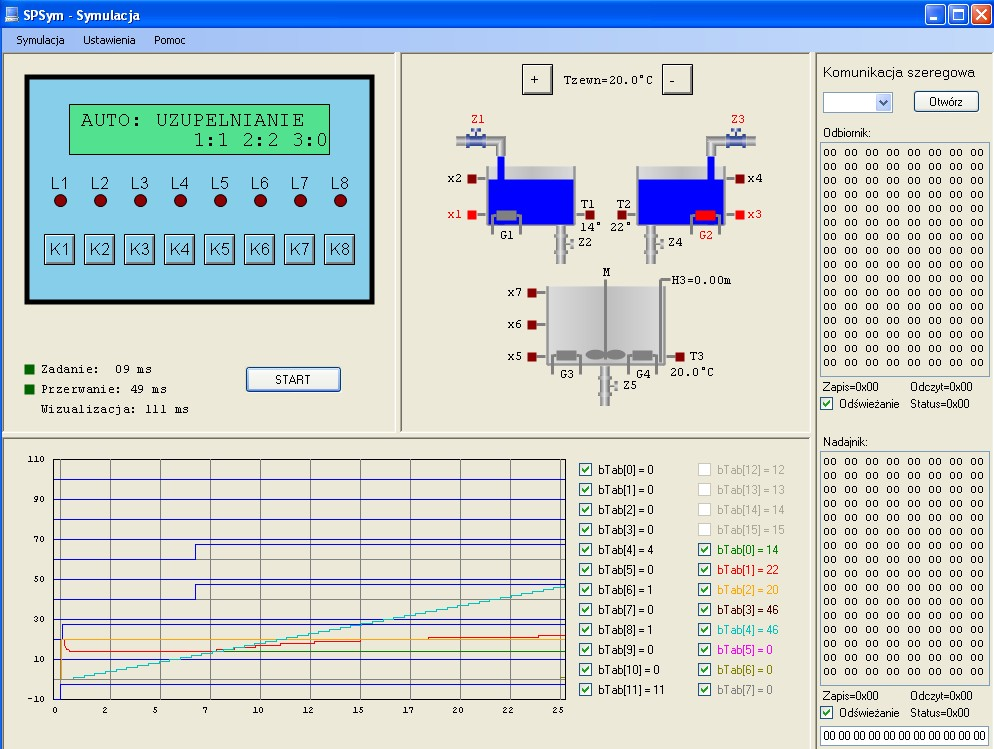
\includegraphics[width=14cm]{figures/ss_zbiorniki/a_start_uzupelnianie.jpg}
    \caption{Tryb automatyczny - rozpoczęcie produkcji, uzupełnianie górnych zbiorników bazy i utwardzacza}
    \label{Fig:a_akryl_start_uzupelnianie}
\end{figure}
\begin{figure}[H]
    \centering
    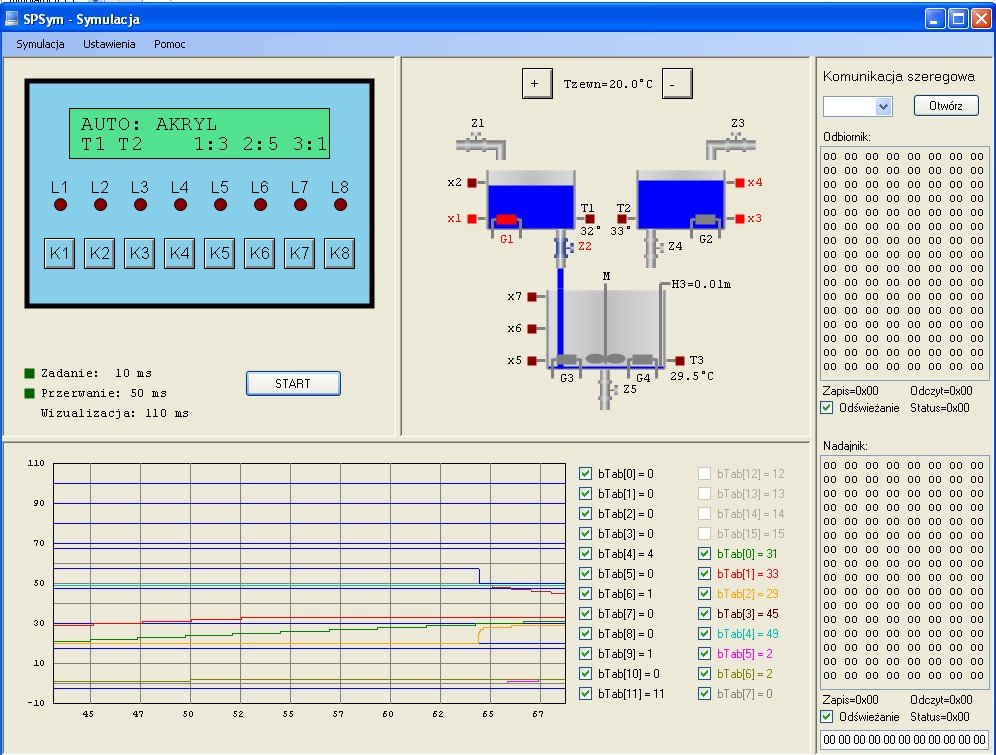
\includegraphics[width=14cm]{figures/ss_zbiorniki/a_akryl_baza.jpg}
    \caption{Tryb automatyczny - produkcja lakieru akrylowego, nalewanie z zaworu Z2 bazy przez 400 cykli}
    \label{Fig:a_akryl_baza}
\end{figure}

\begin{figure}[H]
    \centering
    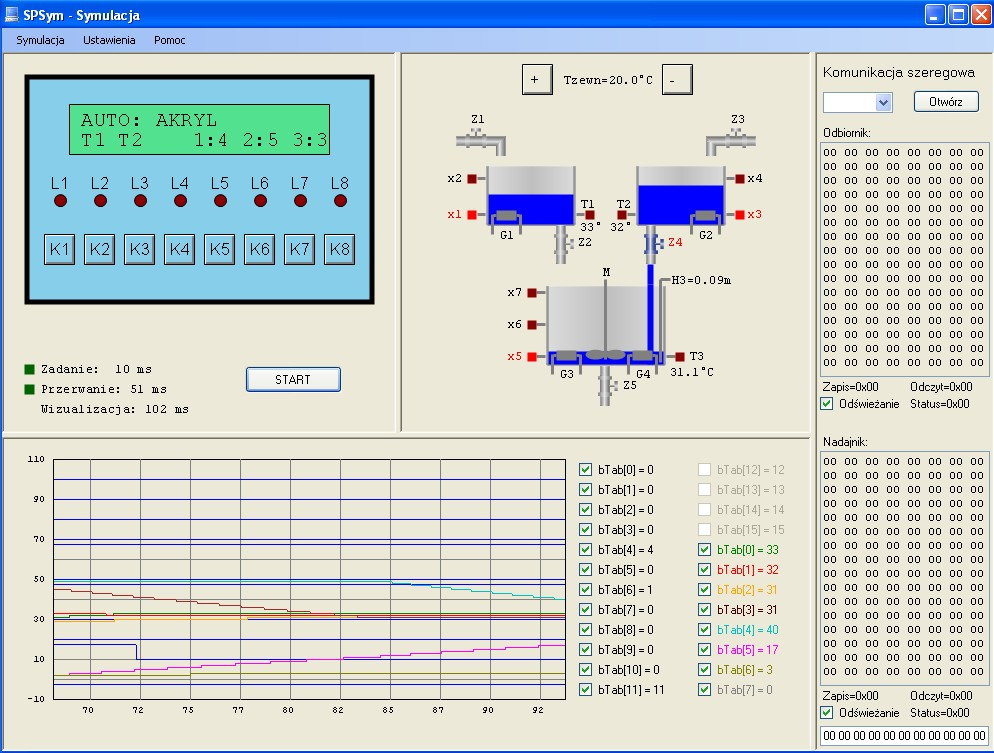
\includegraphics[width=14cm]{figures/ss_zbiorniki/a_akryl_utwardzacz.jpg}
    \caption{Tryb automatyczny - produkcja lakieru akrylowego, nalewanie z zaworu Z4 bazy przez 200 cykli}
    \label{Fig:a_akryl_utwardzacz}
\end{figure}

\begin{figure}[H]
    \centering
    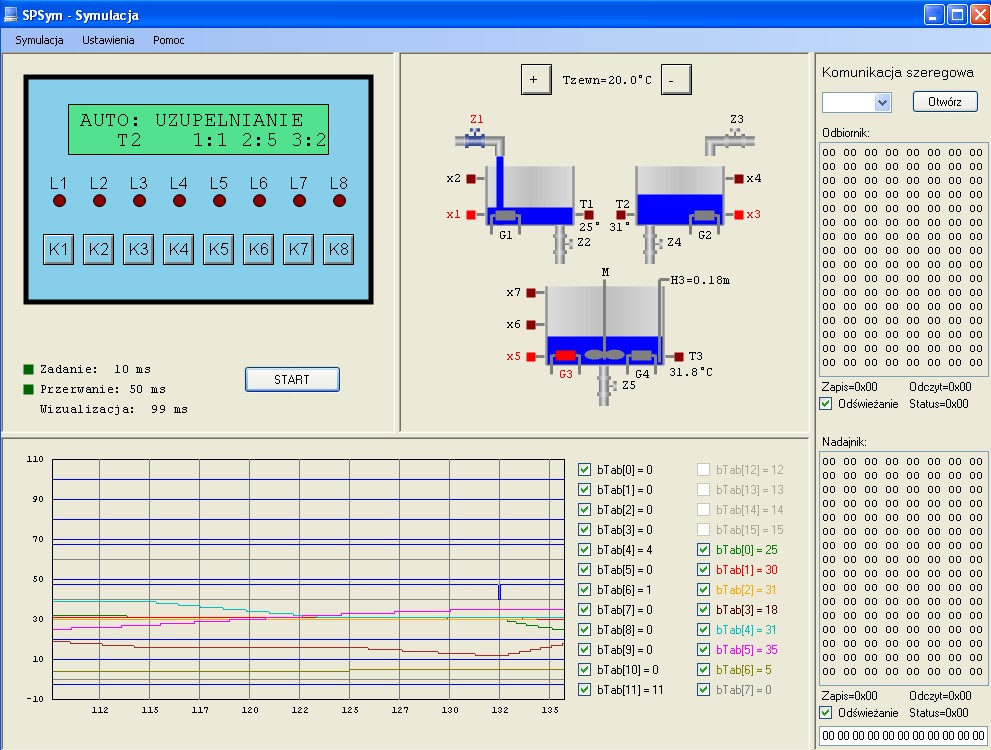
\includegraphics[width=14cm]{figures/ss_zbiorniki/a_akryl_uzupelnianie_brak_skladnikow.jpg}
    \caption{Tryb automatyczny - produkcja lakieru akrylowego, pauza z powodu uzupełniania braków w zbiorniu nr 1}
    \label{Fig:a_akryl_uzupelnianie_brak_skladnikow}
\end{figure}

\begin{figure}[H]
    \centering
    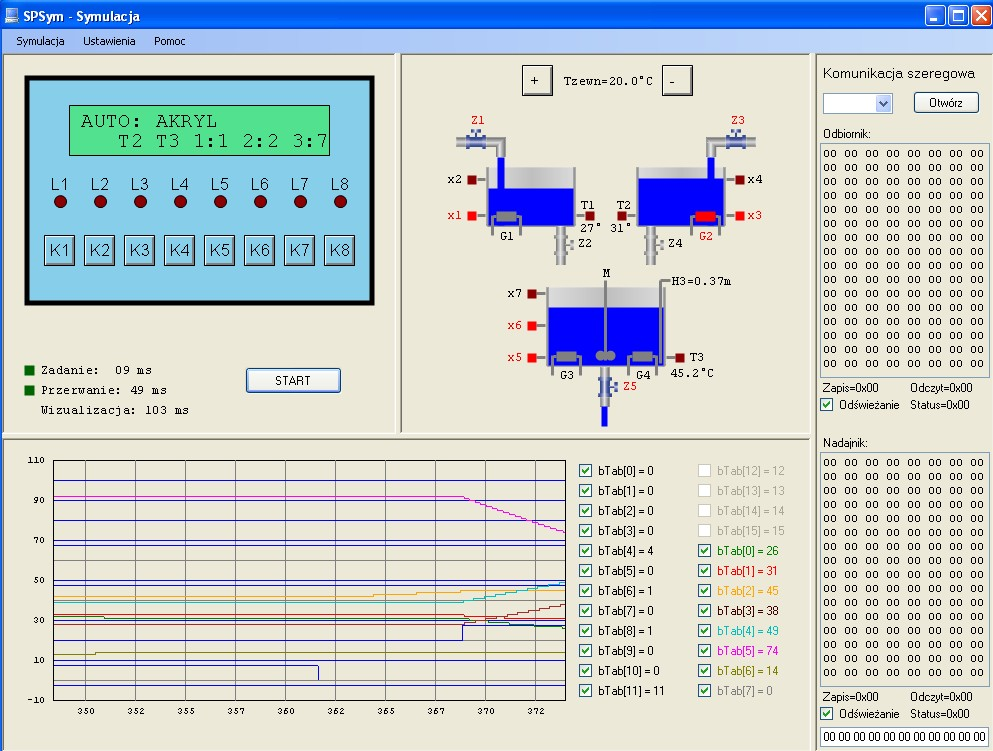
\includegraphics[width=14cm]{figures/ss_zbiorniki/a_akryl_wylewanie.jpg}
    \caption{Tryb automatyczny - produkcja lakieru akrylowego, rozlewanie gotowej mieszaniny przez zawór Z5 oraz uzupełnianie górnych zbiorników}
    \label{Fig:a_akryl_wylewanie}
\end{figure}

Podobnie jak w przypadku lakieru akrylowego, wygląda tworzenie lakieru poliuretanowego, z tą różnicą, że nalewanie utwardzacza trwa tylko 100 cykli, a nie 200. Poniżej przedstawiono zrzuty ekranu z tego procesu:
\begin{figure}[H]
    \centering
    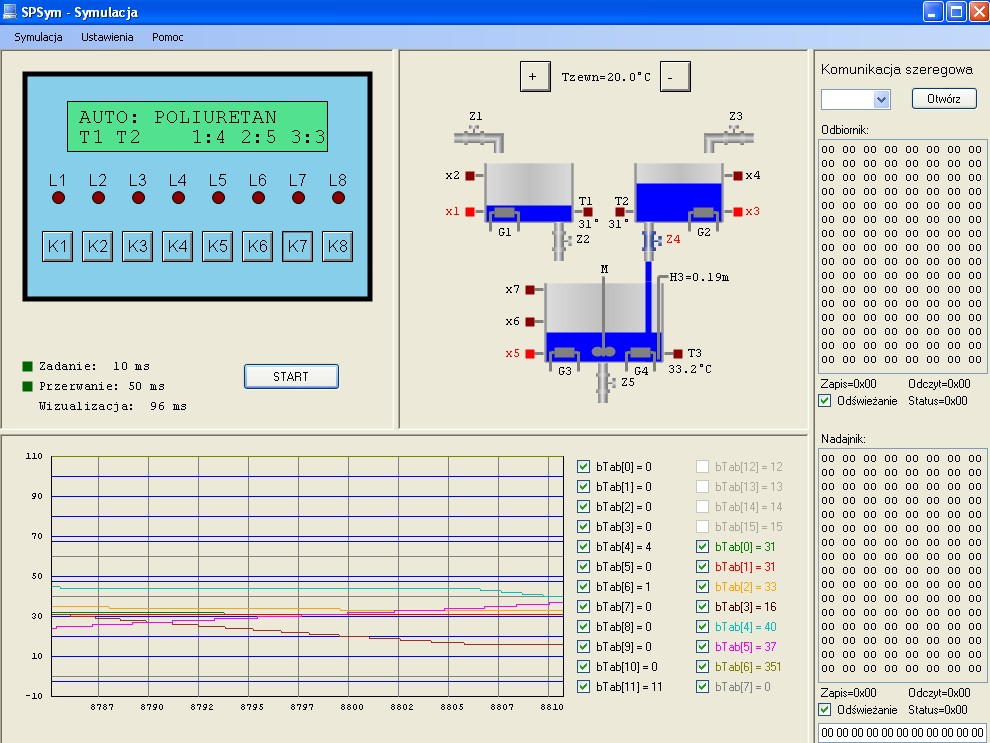
\includegraphics[width=14cm]{figures/ss_zbiorniki/a_poliu_baza.jpg}
        \caption{Tryb automatyczny - produkcja lakieru poliuretanowego, nalewanie z zaworu Z4 utwardzacza przez 100 cykli}
        \label{Fig:a_poliu_utwardzacz}
\end{figure}

\subsection{Tryb manualny}
\begin{figure}[H]
    \centering
    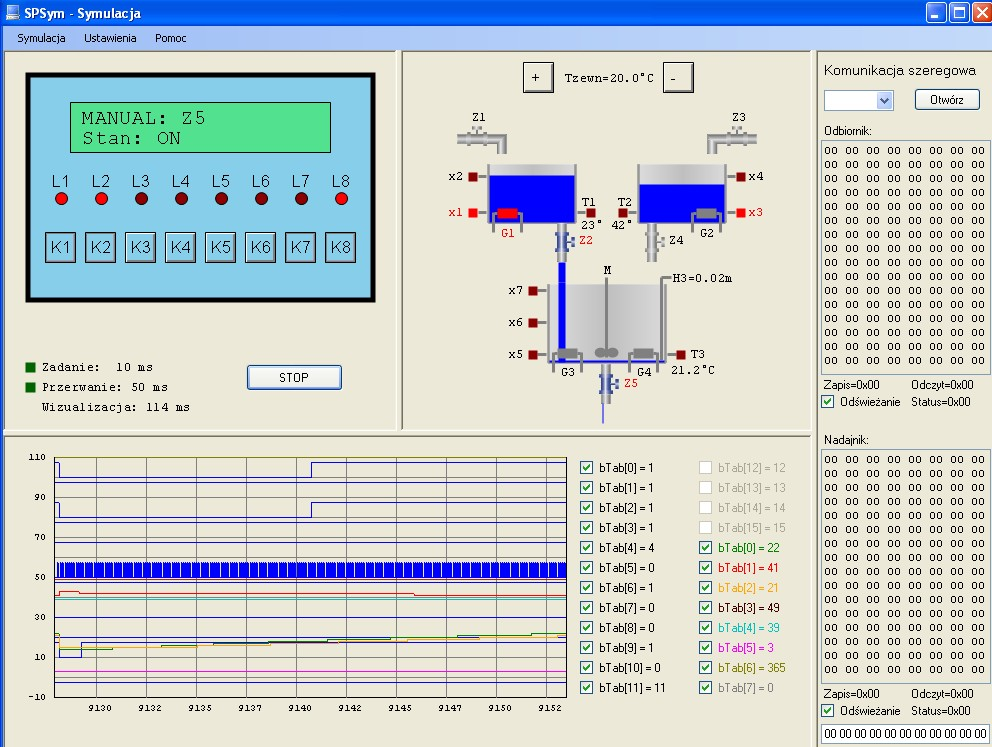
\includegraphics[width=14cm]{figures/ss_zbiorniki/m.jpg}
        \caption{Tryb manualny - użytkownik poprzez panel samodnielnie decyduje o stanach wyjść, jedynym ograniczeniem są zabezpieczenia}
        \label{Fig:m_manual}
\end{figure}

\section*{Podsumowanie}
Podczas realizacji projektu udało się stworzyć kompletny system kaskady zbiorników do mieszania lakierów samochodowych, który spełnia wszystkie założenia funkcjonalne. System działa zarówno w trybie automatycznym, jak i manualnym, a zastosowane zabezpieczenia skutecznie chronią przed niepożądanymi stanami. Projekt pozwolił na praktyczne zastosowanie wiedzy z zakresu systemów wbudowanych. Dodatkowo, implementacja została przeprowadzona z dbałością o czytelność kodu, zasady projektowania automatów Moore'a oraz rygorystyczną zgodność z wymaganiami projektowymi. W przyszłości można rozważyć rozszerzenie funkcjonalności o dodatkowe tryby pracy, bardziej zaawansowane interfejsy użytkownika lub integrację z systemami zewnętrznymi. Kluczowym elementem projektu było wprowadzenie realnej logiki przemysłowej do symulacji, co pozwoliło na lepsze zrozumienie procesów automatyki i sterowania.

\begin{thebibliography}{9}
    \bibitem{wyklady} Świder Z.: \textit{Materiały wykładowe z przedmiotu "Systemy wbudowane"}. Politechnika Rzeszowska, semestr letni 2025/2026.
    \bibitem{Ksiazka} Świder Z., Stec A., Pelc L. Cisek J., Mikluszka W., Śnieżek M.: \textit{Sterowanie mikroprocesorowe}, OWPRz, Rzeszów 2002.
    \bibitem{wymagania} Stec A.: \textit{Wytyczne do projektu nr 1 z przedmiotu "Systemy wbudowane"}. Politechnika Rzeszowska, 2026.
    \bibitem{wymagania} Stec A.: \textit{Dodatkowe uwagi i wytyczne do projektu nr 1 z przedmiotu "Systemy wbudowane"}. Politechnika Rzeszowska, 2026.
    \bibitem{upol_tds} U-POL: \textit{Technical Data Sheet: UP2872V S2087V 2.1VOC Compliant Clear Coat (4:1)}. 2011.
    \bibitem{mipa_tds} Mipa: \textit{Technical Data Sheet: Mipa OC 2K-PUR-Acrylic Car Refinishing Paint}. Wersja US 1025.
\end{thebibliography}

\end{document}